\documentclass[xcolor=dvipsnames,serif,10pt]{beamer}

\usepackage{beamerthemesplit}
\usepackage{media9}
\usepackage{graphics}
\usepackage{graphicx}
\usepackage{hyperref}
\usepackage[normalem]{ulem}
%\usefonttheme{professionalfonts}
%\usepackage{times}
\usepackage{rotating}
\usepackage{tikz}
\usepackage{amsmath,cancel}
\usepackage{mathtools}
\usepackage{verbatim}
\usetikzlibrary{arrows,shapes}
\usepackage{listings}
\usepackage[]{geometry}
\usepackage{ifxetex}
\ifxetex{%
  \usepackage{fontspec}
  \setmainfont{Linux Libertine O} % or any font on your system
  \newfontfamily\quotefont[Ligatures=TeX]{Linux Libertine O} % or any font on your system
\else
  \usepackage[T1]{fontenc}
  \usepackage{libertine} % or any other font package (or none)
  \newcommand*\quotefont{\fontfamily{fxl}} % selects Libertine for quote font
\fi
\usepackage{framed}
\usepackage{booktabs}

\usepackage{soul}
\usetikzlibrary{calc}
\usetikzlibrary{decorations.pathmorphing}
\usetikzlibrary{decorations.text}
\usetikzlibrary{calc,shapes.callouts,shapes.arrows,arrows}
\makeatletter

\newcommand{\defhighlighter}[3][]{%
  \tikzset{every highlighter/.style={color=#2, fill opacity=#3, #1}}%
}

\defhighlighter{yellow}{.5}

\newcommand{\highlight@DoHighlight}{
  \fill [ decoration = {random steps, amplitude=1pt, segment length=15pt}
        , outer sep = -15pt, inner sep = 0pt, decorate
        , every highlighter, this highlighter ]
        ($(begin highlight)+(0,8pt)$) rectangle ($(end highlight)+(0,-3pt)$) ;
}

\newcommand{\highlight@BeginHighlight}{
  \coordinate (begin highlight) at (0,0) ;
}

\newcommand{\highlight@EndHighlight}{
  \coordinate (end highlight) at (0,0) ;
}

\newdimen\highlight@previous
\newdimen\highlight@current

\DeclareRobustCommand*\highlight[1][]{%
  \tikzset{this highlighter/.style={#1}}%
  \SOUL@setup
  %
  \def\SOUL@preamble{%
    \begin{tikzpicture}[overlay, remember picture]
      \highlight@BeginHighlight
      \highlight@EndHighlight
    \end{tikzpicture}%
  }%
  %
  \def\SOUL@postamble{%
    \begin{tikzpicture}[overlay, remember picture]
      \highlight@EndHighlight
      \highlight@DoHighlight
    \end{tikzpicture}%
  }%
  %
  \def\SOUL@everyhyphen{%
    \discretionary{%
      \SOUL@setkern\SOUL@hyphkern
      \SOUL@sethyphenchar
      \tikz[overlay, remember picture] \highlight@EndHighlight ;%
    }{%
    }{%
      \SOUL@setkern\SOUL@charkern
    }%
  }%
  %
  \def\SOUL@everyexhyphen##1{%
    \SOUL@setkern\SOUL@hyphkern
    \hbox{##1}%
    \discretionary{%
      \tikz[overlay, remember picture] \highlight@EndHighlight ;%
    }{%
    }{%
      \SOUL@setkern\SOUL@charkern
    }%
  }%
  %
  \def\SOUL@everysyllable{%
    \begin{tikzpicture}[overlay, remember picture]
      \path let \p0 = (begin highlight), \p1 = (0,0) in \pgfextra
        \global\highlight@previous=\y0
        \global\highlight@current =\y1
      \endpgfextra (0,0) ;
      \ifdim\highlight@current < \highlight@previous
        \highlight@DoHighlight
        \highlight@BeginHighlight
      \fi
    \end{tikzpicture}%
    \the\SOUL@syllable
    \tikz[overlay, remember picture] \highlight@EndHighlight ;%
  }%
  \SOUL@
}
\makeatother


% wrap everything in its own environment
\newenvironment{shadequote}%
{\begin{quote}\openquote}
{\hfill\closequote\end{quote}}

\newcommand{\arrowthis}[2]{
        \tikz[remember picture,baseline]{\node[anchor=base,inner sep=0,outer sep=0]%
        (#1) {\underline{#1}};
        \node[overlay,single arrow,draw=none,fill=red!50,anchor=tip,rotate=60] 
        at (#1.south) {#2};}%
    }%

\newcommand{\speechthis}[2]{
        \tikz[remember picture,baseline]{\node[anchor=base,inner sep=0,outer sep=0]%
        (#1) {\underline{#1}};\node[overlay,ellipse callout,fill=blue!50] 
        at ($(#1.north)+(-.5cm,0.8cm)$) {#2};}%
    }%

\newcommand{\bubblethis}[2]{
        \tikz[remember picture,baseline]{\node[anchor=base,inner sep=0,outer sep=0]%
        (#1) {\underline{#1}};\node[overlay,cloud callout,callout relative pointer={(0.2cm,-0.7cm)},%
        aspect=2.5,fill=yellow!90] at ($(#1.north)+(-0.5cm,1.6cm)$) {#2};}%
    }%

\newcommand{\pointthis}[2]{
        \tikz[remember picture,baseline]{\node[anchor=base,inner sep=0,outer sep=0]%
        (#1) {\underline{#1}};\node[overlay,rectangle callout,%
        callout relative pointer={(0.2cm,0.7cm)},fill=green!50] at ($(#1.north)+(-.5cm,-1.4cm)$) {#2};}%
        }%


\usetikzlibrary{mindmap,backgrounds}

    \definecolor{listcomment}{rgb}{0.0,0.5,0.0}
    \definecolor{listkeyword}{rgb}{0.0,0.0,0.5}
    \definecolor{listnumbers}{gray}{0.65}
    \definecolor{listlightgray}{gray}{0.9}
    \definecolor{listwhite}{gray}{1.0}


\usetheme[secheader]{Boadilla}
\useoutertheme{miniframes}
\useinnertheme{circles}
\usecolortheme{myct}
\usepackage[latin1]{inputenc}

\graphicspath{{Figures/}{../Figures/}}

\setlength{\tabcolsep}{1pt}

\newcommand\fontvi{\fontsize{6}{8}\selectfont}
\newcommand{\ColIndent}{\hspace{\labelwidth}\hspace{\labelsep}\hspace{\labelsep}\hspace{\labelsep}\hspace{\labelsep}}

\usetikzlibrary{backgrounds}
\usetikzlibrary{positioning}
\makeatletter


%%%%%%%%%%%%%%%%%%%%%%%%%%%%%
%%  Title slide
%%%%%%%%%%%%%%%%%%%%%%%%%%%%%

\title[Longitudinal assessment]{Longitudinal assessment of treatment effects on pulmonary ventilation using 1H/3He MRI multivariate templates}
\author[N. Tustison]{%
  N. J. Tustison$^{1}$, B. Contrella$^{1}$, T. A. Altes$^{1}$, B. B. Avants$^{2}$, E. E. de Lange$^{1}$, J. P. Mugler III$^{1}$
  }
\date[SPIE 2013:  Orlando, FL]{}
\institute[ntustison@virginia.edu]{
  $^{1}$Department of Radiology and Medical Imaging, University of Virginia \\
  $^{2}$Penn Image and Computing Science Laboratory, University of Pennsylvania
}
%\pgfdeclaremask{fsu}{fsu_logo_ybkgrd}
%\pgfdeclareimage[width=1cm]{logo}{ants_logo}
%\logo{\vbox{\vskip0.1cm\hbox{\pgfuseimage{logo}}}}

%\logo{
%  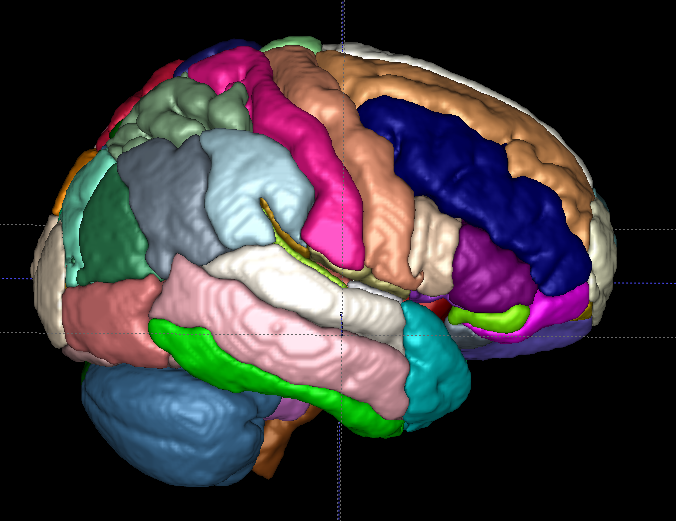
\includegraphics[height=0.8cm]{brain2.png}
%  
\includegraphics[height=0.8cm]{itkLogo.jpg}
%  }

\begin{document}

\tikzstyle{every picture}+=[remember picture]

\frame{\titlepage}


%%%%%%%%%%%%%%%%%%%%%%%%%%%%%
%% Segmentation review
%%%%%%%%%%%%%%%%%%%%%%%%%%%%%

\begin{frame}{Previously\ldots}

\begin{center}
  \begin{tabular*}{0.5\textwidth}{l@{\extracolsep{\fill}}c@{\extracolsep{\fill}}c}
    \toprule
    Rater & Sensitivity & Specificity\\
    \midrule
    Atropos & 0.898 & 0.905 \\
    Radiologist 1 & 0.743 & 0.897 \\
    Radiologist 2 & 0.501 & 0.985 \\
    Radiologist 3 & 0.898 & 0.848 \\
    First author & 0.600 & 0.984 \\
    K-means      & 0.973 & 0.734 \\
    \bottomrule
  \end{tabular*}
\end{center}
  
\end{frame}

%%%%%%%%%%%%%%%%%%%%%%%%%%%%%
%% 4-D Atropos
%%%%%%%%%%%%%%%%%%%%%%%%%%%%%

\tikzset{
%Define standard arrow tip
>=stealth'
}

\begin{frame}{Longitudinal segmentation}

 \begin{tikzpicture}[scale=1]
   \path[use as bounding box] (0,6) rectangle (-1,0);

    % A grid can be useful when defining coordinates
    \draw[step=2mm, middlecolour, thin] (0,0) grid (9.8,5.8); 
%    \draw[step=5mm, black] (0,0) grid (10,6.5); 


   \draw[<-|,thick] (3.25,-0.5) -- node[sloped,midway,above] {\footnotesize Time point} +(-4,4);
   \filldraw (2.85,-0.1) circle (2pt);
   \filldraw (2.05,0.7) circle (2pt);
   \filldraw (1.25,1.5) circle (2pt);
   \filldraw (0.45,2.3) circle (2pt);
   \filldraw (-0.35,3.1) circle (2pt);

    \node[left] at (-0.35,3.1) {\scriptsize $t=1$}; 
    \node[left] at (0.45,2.3) {\scriptsize $t=2$}; 
    \node[left] at (1.25,1.5) {\scriptsize $t=3$}; 
    \node[left] at (2.05,0.7) {\scriptsize $t=4$}; 
    \node[left] at (2.85,-0.1) {\scriptsize $t=5$}; 

   \path[->,rounded corners=0.1cm] node[text width=1.5cm,xshift=1.0cm,yshift=4.15cm]  { 
  		  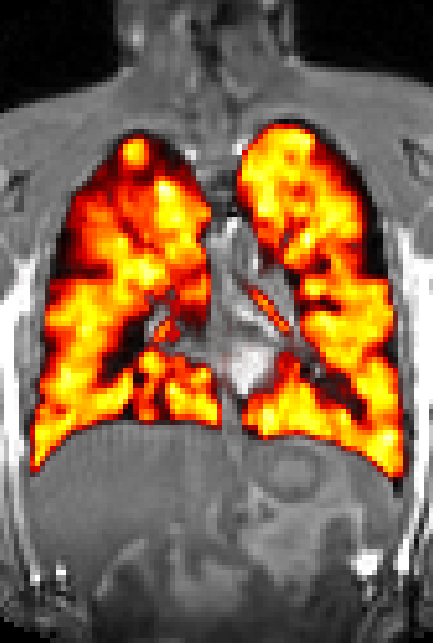
\includegraphics[width=1.5cm]{subject2_timePoint1.png}
			};
   \path[->,rounded corners=0.1cm] node[text width=1.5cm,xshift=1.8cm,yshift=3.35cm]  { 
  		  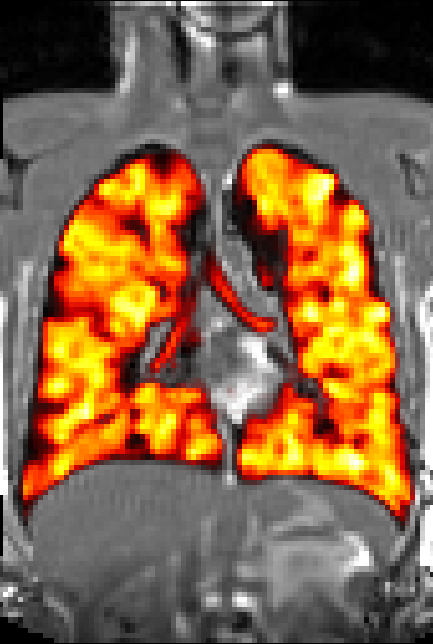
\includegraphics[width=1.5cm]{subject2_timePoint2.png}
			};
   \path[->,rounded corners=0.1cm] node[text width=1.5cm,xshift=2.6cm,yshift=2.55cm]  { 
  		  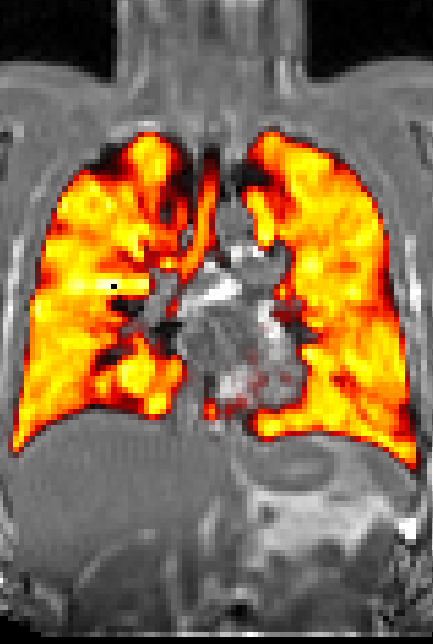
\includegraphics[width=1.5cm]{subject2_timePoint3.png}
			};
   \path[->,rounded corners=0.1cm] node[text width=1.5cm,xshift=3.5cm,yshift=1.75cm]  { 
  		  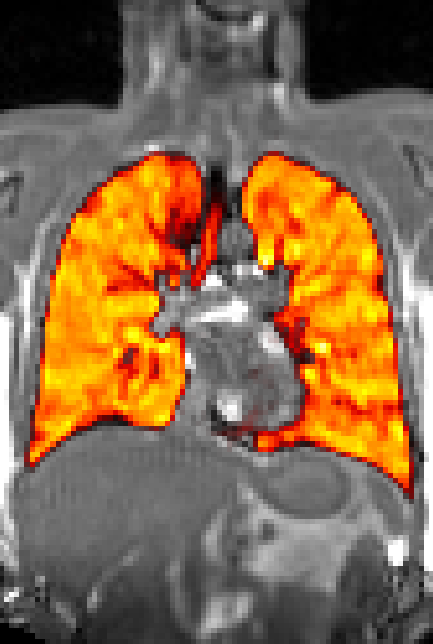
\includegraphics[width=1.5cm]{subject2_timePoint4.png}
			};
   \path[->,rounded corners=0.1cm] node[text width=1.5cm,xshift=4.2cm,yshift=0.95cm]  { 
  		  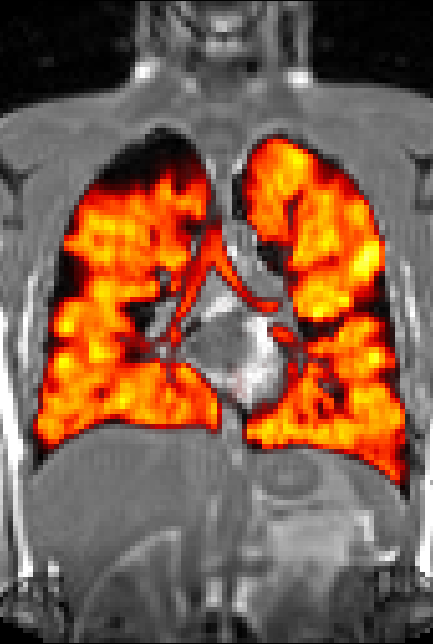
\includegraphics[width=1.5cm]{subject2_timePoint5.png}
			};

   \path[->,rounded corners=0.1cm] node[text width=1.5cm,xshift=7.0cm,yshift=4.15cm]  { 
  		  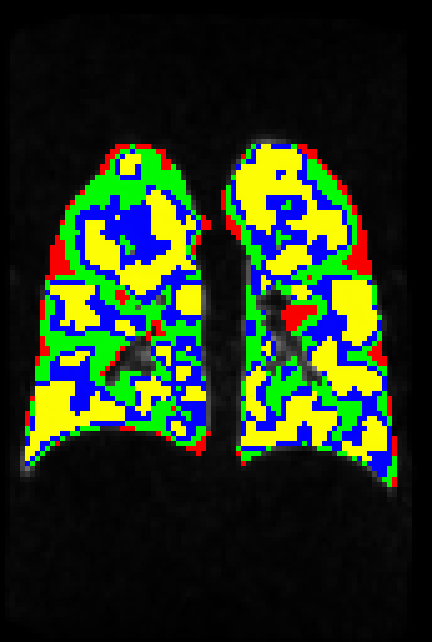
\includegraphics[width=1.5cm]{subject2_timePoint1_atropos.png}
			};
   \path[->,rounded corners=0.1cm] node[text width=1.5cm,xshift=7.8cm,yshift=3.35cm]  { 
  		  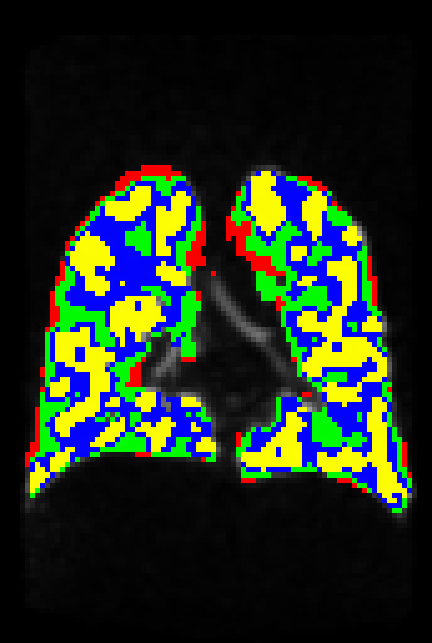
\includegraphics[width=1.5cm]{subject2_timePoint2_atropos.png}
			};
   \path[->,rounded corners=0.1cm] node[text width=1.5cm,xshift=8.6cm,yshift=2.55cm]  { 
  		  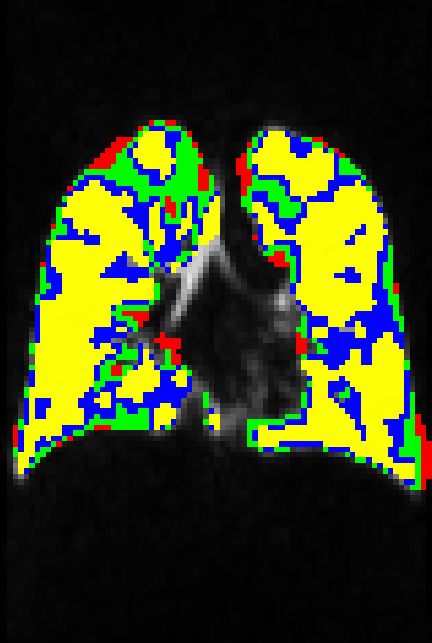
\includegraphics[width=1.5cm]{subject2_timePoint3_atropos.png}
			};
   \path[->,rounded corners=0.1cm] node[text width=1.5cm,xshift=9.5cm,yshift=1.75cm]  { 
  		  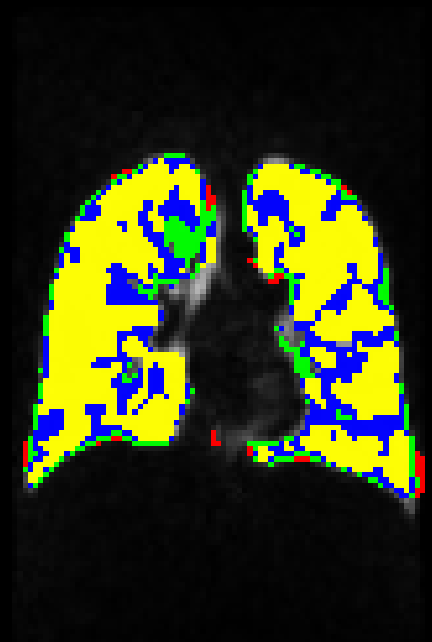
\includegraphics[width=1.5cm]{subject2_timePoint4_atropos.png}
			};
   \path[->,rounded corners=0.1cm] node[text width=1.5cm,xshift=10.2cm,yshift=0.95cm]  { 
  		  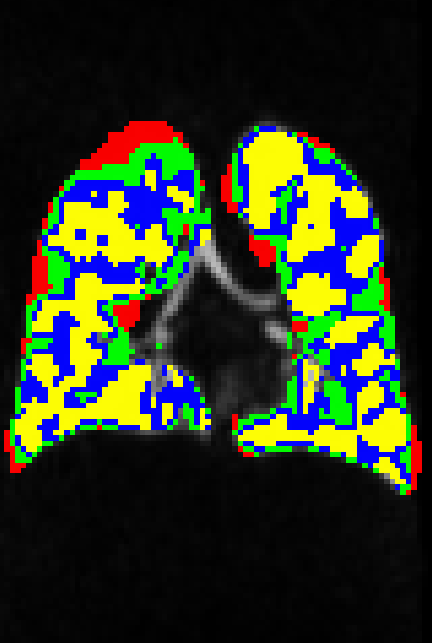
\includegraphics[width=1.5cm]{subject2_timePoint5_atropos.png}
			};

%   \draw[->, >=latex, blue!20!white, line width=72pt] (4, 16) � node [black,sloped]            {Optimization} +(-45:17cm);			

   \draw[->, thick, dashed] (3, 4) -- node [text width= 3cm,above, midway, xshift=0.25cm]  {\scriptsize Intensity normalization and 4-D segmentation} +(3,0); 

    \end{tikzpicture}


\end{frame}

%%%%%%%%%%%%%%%%%%%%%%%%%%%%%
%%  Expected ventilation
%%%%%%%%%%%%%%%%%%%%%%%%%%%%%

\begin{frame}{Expected ventilation}

 \begin{tikzpicture}[scale=1]
   \path[use as bounding box] (0,6) rectangle (-1,0);

   \path[->,rounded corners=0.1cm] node[yshift = 5.5cm] (pos1) { 
  		  
\includegraphics[width=1.5cm]{subject2_526_posterior1.png}
			};
   \path[->,rounded corners=0.1cm] node[below of=pos1, yshift=-0.5cm] (pos2) { 
  		  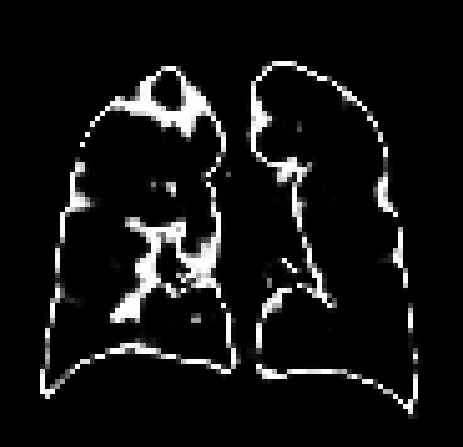
\includegraphics[width=1.5cm]{subject2_526_posterior2.png}
			};
   \path[->,rounded corners=0.1cm] node[below of=pos2, yshift=-0.5cm] (pos3) { 
  		  
\includegraphics[width=1.5cm]{subject2_526_posterior3.png}
			};
   \path[->,rounded corners=0.1cm] node[below of=pos3, yshift=-0.5cm] (pos4) { 
  		  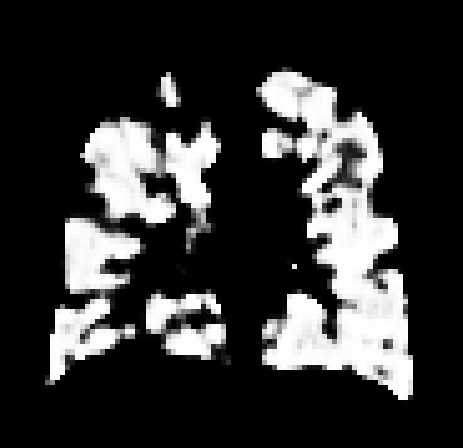
\includegraphics[width=1.5cm]{subject2_526_posterior4.png}
			};
   \path[->,rounded corners=0.1cm] node[right of=pos2, xshift=3.75cm, yshift=-0.75cm] (eqn) { 
    $EV_{v} = \sum_{l=1}^4 l \times \mathrm{Pr}( l | I_v )$ 
			};
   \path[-,rounded corners=0.1cm] node[right of=pos2, xshift=8cm, yshift=-0.75cm] (ev) { 
  		  
\includegraphics[width=3cm]{subject2_526_ev.png}
			};

   \path[->,thick, color = red] (pos1.east) edge [out=0, in=180] node[xshift=-0.75cm,yshift=1.3cm] {\scriptsize $l=1$} (eqn.west);			  
   \path[->,thick, color = green] (pos2.east) edge [out=0, in=180] node[xshift=-0.75cm,yshift=0.55cm] {\scriptsize $l=2$} (eqn.west);			  
   \path[->,thick, color = blue] (pos3.east) edge [out=0, in=180] node[xshift=-0.75cm,yshift=-0.5cm] {\scriptsize $l=3$}(eqn.west);			  
   \path[->,thick, color = yellow] (pos4.east) edge [out=0, in=180] node[xshift=-0.75cm,yshift=-1.25cm] {\scriptsize $l=4$}(eqn.west);			  
   \path[->,thick] (eqn.east) edge [out=0, in=180] (ev.west);			  



 \end{tikzpicture}

%\begin{block}{}
%  \begin{align*} 
%    EV_{v} = \sum_{l=1}^L l \times \mathrm{Pr}( l | I_v ) \\
%  \end{align*}
%\end{block}

\end{frame}

%%%%%%%%%%%%%%%%%%%%%%%%%%%%%
%%  template generation
%%%%%%%%%%%%%%%%%%%%%%%%%%%%%

\begin{frame}{Template generation}

Given $\{I_1^{1H},I_1^{3He},\ldots,I_5^{1H},I_5^{3He}\}$, template generation involves finding:
\begin{itemize}
  \item the set of paired diffeomorphic transformations $\left\{ \left(\phi_1,\phi_1^{-1}\right),\ldots, \left(\phi_5,\phi_5^{-1}\right) \right\}$,
  \item optimal appearance template, $J^{1H}$ and $J^{3He}$, and
  \item the corresponding coordinate system, $\psi(\mathbf{x})$
\end{itemize}
which minimize$^\dagger$
\begin{block}{}
\begin{align*}
C &= \sum_{i=1}^5 \left[ 
             D\left( \psi((\mathbf{x})), \phi(\mathbf{x}, 1)\right)
             + \Pi_1\left( I_m^{1H} \left( \phi_2^m (\mathbf{x},0.5 )\right), 
                         J^{1H}\left(\phi_1^m(\mathbf{x},0.5)\right)\right) 
             \right. \\
              &+ \left.\Pi_2\left( I_m^{3He} \left( \phi_2^m (\mathbf{x},0.5 )\right),
                          J^{3He}\left(\phi_2^m(\mathbf{x},0.5)\right)\right)
            \right]\\
\end{align*}
{ \scriptsize $^\dagger$implemented in \texttt{antsMultivariateTemplateConstruction.sh}}
\end{block}

\end{frame}

%%%%%%%%%%%%%%%%%%%%%%%%%%%%%
%%  He3/H1 template
%%%%%%%%%%%%%%%%%%%%%%%%%%%%%

\begin{frame}{He3/H1 longitudinal template}

\begin{center}
  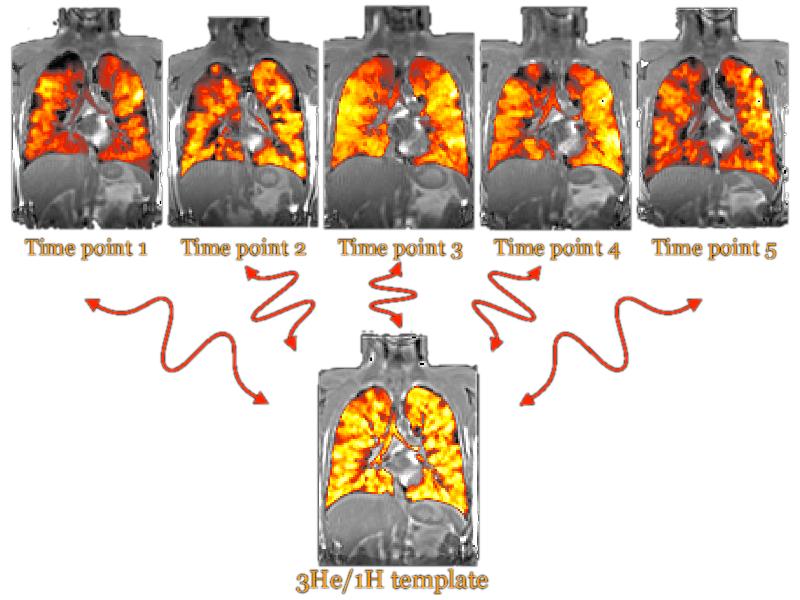
\includegraphics[width=9cm]{He3H1template.png} 
\end{center}

\end{frame}


%%%%%%%%%%%%%%%%%%%%%%%%%%%%%
%%  Correlation analysis
%%%%%%%%%%%%%%%%%%%%%%%%%%%%%

\tikzset{
%Define standard arrow tip
>=stealth',
%Define style for different line styles
help lines/.style={dashed, thick},
axis/.style={<->,thick},
important line/.style={thick},
connection/.style={thick, dotted},
}

\begin{frame}{Correlation analysis}


%\begin{tikzpicture}[node distance=1cm, auto,>=latex', thin]
%    % We need to set at bounding box first. Otherwise the diagram
%    % will change position for each frame.

 \begin{tikzpicture}[scale=1]
   \path[use as bounding box] (0,6) rectangle (-1,0);

    % A grid can be useful when defining coordinates
    \draw[step=2mm, middlecolour, thin] (0,0) grid (9.8,5.8); 
%    \draw[step=5mm, black] (0,0) grid (10,6.5); 

    % Axis
    \coordinate (y) at (0,6);
    \coordinate (x) at (10,0);
    \draw[<->,thick] (y) node[above] {\scriptsize \em Expected ventilation} -- (0,0) --  (x) node[right]
    {\scriptsize \em Time};

    \coordinate (y1) at (0, 1.25);
    \coordinate (y2) at (0, 2.5);
    \coordinate (y3) at (0, 3.75);
    \coordinate (y4) at (0, 5);

    \node[left] at (y1) {1}; 
    \node[left] at (y2) {2}; 
    \node[left] at (y3) {3}; 
    \node[left] at (y4) {4}; 

    \coordinate (x1) at (1.75, 0);
    \coordinate (x2) at (3.5, 0);
    \coordinate (x3) at (5.25, 0);
    \coordinate (x4) at (7, 0);
    \coordinate (x5) at (8.75, 0);

    \node[below] at (x1) {1}; 
    \node[below] at (x2) {2}; 
    \node[below] at (x3) {3}; 
    \node[below] at (x4) {4}; 
    \node[below] at (x5) {5}; 

    \path[->,rounded corners=0.1cm] node[text width=1.5cm,xshift=1.75cm,yshift=1.15cm] (t1) { 
			  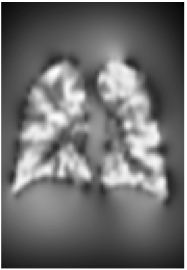
\includegraphics[width=1.5cm]{timePoint1.png} \\
			  };
    \draw[thick,red] ([xshift=-0.35cm,yshift=1.5cm]x1) circle (1pt);
    
    \path[->,rounded corners=0.1cm] node[text width=1.5cm,xshift=3.5cm,yshift=1.15cm] (t2) { 
			  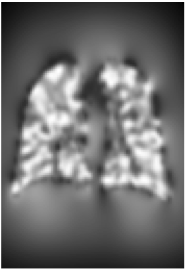
\includegraphics[width=1.5cm]{timePoint2.png} \\
			  };
    \draw[thick,green] ([xshift=-0.35cm,yshift=1.5cm]x2) circle (1pt);
    
    \path[->,rounded corners=0.1cm] node[text width=1.5cm,xshift=5.25cm,yshift=1.15cm] (t3) { 
			  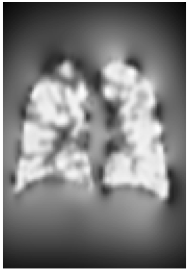
\includegraphics[width=1.5cm]{timePoint3.png} \\
			  };
    \draw[thick,blue] ([xshift=-0.35cm,yshift=1.5cm]x3) circle (1pt);

    \path[->,rounded corners=0.1cm] node[text width=1.5cm,xshift=7cm,yshift=1.15cm] (t4) { 
			  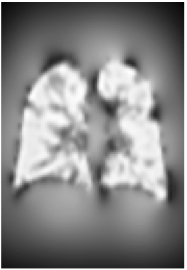
\includegraphics[width=1.5cm]{timePoint4.png} \\
			  };
    \draw[thick,orange] ([xshift=-0.35cm,yshift=1.5cm]x4) circle (1pt);

    \path[->,rounded corners=0.1cm] node[text width=1.5cm,xshift=8.75cm,yshift=1.15cm] (t5) { 
			  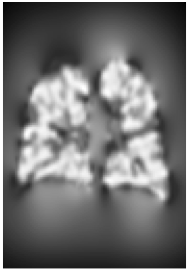
\includegraphics[width=1.5cm]{timePoint5.png} \\
			  };
    \draw[thick,violet] ([xshift=-0.35cm,yshift=1.5cm]x5) circle (1pt);

  
    % Let us define some coordinates
    \path
    coordinate (c0) at (1.75, 2.5)
    coordinate (c1) at (3.5, 2.5)
    coordinate (c2) at (5.25,5)
    coordinate (c3) at (7,5)
    coordinate (c4) at (8.75,3.75);

    \draw[dashed,very thick] (c0) -- (c1) -- (c2)  -- (c3) -- node[sloped,midway,below] {\tiny simplified hypothesis} (c4);

%    \draw[dashed,very thick] (c0) -- (c1) -- (c2) node[xshift=0.9cm,yshift=-0.25cm] {\tiny simplified hypothesis} -- (c3) -- (c4);
    
    \draw[very thick,red] ([yshift=1.2pt]c0) circle (3pt);
    \draw[very thick,green] ([yshift=17pt]c1) circle (3pt);
    \draw[very thick,blue] ([yshift=5pt]c2) circle (3pt);
    \draw[very thick,orange] ([yshift=12pt]c3) circle (3pt);
    \draw[very thick,violet] ([yshift=40pt]c4) circle (3pt);
    
    \draw[|<->|,dotted,thick] ([xshift=-10pt,yshift=17pt]c1) -- node[sloped,midway,above] {\tiny magnitude difference} +(0,2.1);


    \end{tikzpicture}


\end{frame}



%%%%%%%%%%%%%%%%%%%%%%%%%%%%%
%%  Subjects 1-4
%%%%%%%%%%%%%%%%%%%%%%%%%%%%%

\begin{frame}{Subjects 1--4}
\begin{center}
    \includemedia[activate=pageopen,
                  width=5.9325cm,
                  height=3.465cm,
                  addresource=VX770-025001-3D.mov,
                  flashvars={%
                    src=VX770-025001-3D.mov%
                    &autoPlay=true%
                    &loop=true%
                    }
                  ]{}{StrobeMediaPlayback.swf}                  
    \includemedia[activate=pageopen,
                  width=5.9325cm,
                  height=3.465cm,
                  addresource=VX770-025002-3D.mov,
                  flashvars={%
                    src=VX770-025002-3D.mov%
                    &autoPlay=true%
                    &loop=true%
                    }
                  ]{}{StrobeMediaPlayback.swf}   \\               
    \includemedia[activate=pageopen,
                  width=5.9325cm,
                  height=3.465cm,
                  addresource=VX770-025003-3D.mov,
                  flashvars={%
                    src=VX770-025003-3D.mov%
                    &autoPlay=true%
                    &loop=true%
                    }
                  ]{}{StrobeMediaPlayback.swf}                  
    \includemedia[activate=pageopen,
                  width=5.9325cm,
                  height=3.465cm,
                  addresource=VX770-025004-3D.mov,
                  flashvars={%
                    src=VX770-025004-3D.mov%
                    &autoPlay=true%
                    &loop=true%
                    }
                  ]{}{StrobeMediaPlayback.swf}             
\end{center}
\end{frame}

%%%%%%%%%%%%%%%%%%%%%%%%%%%%%
%%  Subjects 5-8
%%%%%%%%%%%%%%%%%%%%%%%%%%%%%

\begin{frame}{Subjects 5--8}
\begin{center}
    \includemedia[activate=pageopen,
                  width=5.9325cm,
                  height=3.465cm,
                  addresource=VX770-025005-3D.mov,
                  flashvars={%
                    src=VX770-025005-3D.mov%
                    &autoPlay=true%
                    &loop=true%
                    }
                  ]{}{StrobeMediaPlayback.swf}                  
    \includemedia[activate=pageopen,
                  width=5.9325cm,
                  height=3.465cm,
                  addresource=VX770-025006-3D.mov,
                  flashvars={%
                    src=VX770-025006-3D.mov%
                    &autoPlay=true%
                    &loop=true%
                    }
                  ]{}{StrobeMediaPlayback.swf}   \\               
    \includemedia[activate=pageopen,
                  width=5.9325cm,
                  height=3.465cm,
                  addresource=VX770-025007-3D.mov,
                  flashvars={%
                    src=VX770-025007-3D.mov%
                    &autoPlay=true%
                    &loop=true%
                    }
                  ]{}{StrobeMediaPlayback.swf}                  
    \includemedia[activate=pageopen,
                  width=5.9325cm,
                  height=3.465cm,
                  addresource=VX770-025008-3D.mov,
                  flashvars={%
                    src=VX770-025008-3D.mov%
                    &autoPlay=true%
                    &loop=true%
                    }
                  ]{}{StrobeMediaPlayback.swf}             
\end{center}
\end{frame}

%%%%%%%%%%%%%%%%%%%%%%%%%%%%%
%%  Test
%%%%%%%%%%%%%%%%%%%%%%%%%%%%%

%\begin{frame}
%\begin{itemize}
%  \item This one is always shown
%  \item<1-> The first time (i.e. as soon as the slide loads)
%  \item<2-> The second time
%  \item<1-> Also the first time
%  \only<1-1> This one is shown at the first time, but it will hide soon (on the next event after the slide loads).
%\end{itemize}
%\end{frame}

%\begin{frame}
%        \frametitle{`Hidden higher-order concepts?'}
%        \begin{itemize}[<+->]
%        \item The truths of arithmetic which are independent of PA in some 
%        sense themselves `{contain} essentially {\color{blue}{hidden higher-order}},
%         or infinitary, concepts'???
%        \item `Truths in the language of arithmetic which \ldots
%        \item   That suggests stronger version of Isaacson's thesis. 
%        \end{itemize}
%\end{frame}
%
%\begin{frame}
% 
%   \begin{block}{This is a Block}
%      This is important information
%   \end{block}
% 
%   \begin{alertblock}{This is an Alert block}
%   This is an important alert
%   \end{alertblock}
% 
%   \begin{exampleblock}{This is an Example block}
%   This is an example 
%   \end{exampleblock}
% 
%\end{frame}

%%%%%%%%%%%%%%%%%%%%%%%%%%%%%
%%  Closing slide
%%%%%%%%%%%%%%%%%%%%%%%%%%%%%

\begin{frame}{}


\begin{tikzpicture}[node distance=1cm, auto,>=latex', thin]
    % We need to set at bounding box first. Otherwise the diagram
    % will change position for each frame.
    \path[->,rounded corners=0.1cm] node[text width=2cm,xshift=-2cm] (ants) { 
        \begin{center}
			  
\includegraphics[width=3.5cm]{ants2.png} \\
        \end{center}
			  };
    \path[->,rounded corners=0.1cm] node[text width=6.5cm, xshift=5.5cm, right of=ants] { 
        \begin{center}
        \begin{block}{Further information}
        \begin{itemize}
          \item \url{http://www.itk.org}
          \item \url{http://www.picsl.upenn.edu/ANTs}
        \end{itemize}
        \end{block}
        \end{center}
			  };
			  
\end{tikzpicture}
\end{frame}

\end{document}